\documentclass[unknownkeysallowed]{beamer}
\usepackage[french,english]{babel}
\usepackage{./tex/sty/beamer_js}
\usepackage{./tex/sty/shortcuts_js}
\addbibresource{./tex/biblio/references_all.bib}
\usepackage{csquotes}
\begin{document}


%%%%%%%%%%%%%%%%%%%%%%%%%%%%%%%%%%%%%%%%%%%%%%%%%%%%%%%%%%%%%%%%%%%%%%%%%%%%%%%
%%%%%%%%%%%%%%%%%%%%%%             Headers               %%%%%%%%%%%%%%%%%%%%%%
%%%%%%%%%%%%%%%%%%%%%%%%%%%%%%%%%%%%%%%%%%%%%%%%%%%%%%%%%%%%%%%%%%%%%%%%%%%%%%%



%%%%%%%%%%%%%%%%%%%%%%%%%%%%%%%%%%%%%%%%%%%%%%%%%%%%%%%%%%%%%%%%%%%%%%%%%%%%%%%
\begin{frame}
\bigskip
\bigskip
\begin{center}{
\LARGE\color{marron}
\textbf{HMMA 307 : Modèles linéaires avancés}
\textbf{ }\\
\vspace{0.5cm}
}

\color{marron}
\textbf{REstricted Maximum Likelihood (REML)}
\end{center}

\vspace{0.5cm}

\begin{center}
\textbf{Ophélie Coiffier} \\
\vspace{0.1cm}
\url{https://github.com/opheliecoiffier/REML}\\
\vspace{0.5cm}
Université de Montpellier \\
\end{center}

\centering
\includegraphics[width=0.13\textwidth]{./images/Logo.pdf}

\end{frame}
%%%%%%%%%%%%%%%%%%%%%%%%%%%%%%%%%%%%%%%%%%%%%%%%%%%%%%%%%%%%%%%%%%%%%%%%%%%%%%%



%%%%%%%%%%%%%%%%%%%%%%%%%%%%%%%%%%%%%%%%%%%%%%%%%%%%%%%%%%%%%%%%%%%%%%%%%%%%%%%
%%%%%%%%%%%%%%%%%%%%%%%%       PLAN      %%%%%%%%%%%%%%%%%%%%%%%%%%%%%%%%%%%%%%
%%%%%%%%%%%%%%%%%%%%%%%%%%%%%%%%%%%%%%%%%%%%%%%%%%%%%%%%%%%%%%%%%%%%%%%%%%%%%%%



%%%%%%%%%%%%%%%%%%%%%%%%%%%%%%%%%%%%%%%%%%%%%%%%%%%%%%%%%%%%%%%%%%%%%%%%%%%%%%%
\begin{frame}{Table of Contents}
\tableofcontents[hideallsubsections]
\end{frame}
%%%%%%%%%%%%%%%%%%%%%%%%%%%%%%%%%%%%%%%%%%%%%%%%%%%%%%%%%%%%%%%%%%%%%%%%%%%%%%%



%%%%%%%%%%%%%%%%%%%%%%%%%%%%%%%%%%%%%%%%%%%%%%%%%%%%%%%%%%%%%%%%%%%%%%%%%%%%%%%
\AtBeginSection[]
{
\begin{frame}<beamer>{Table of Contents}
\tableofcontents[currentsubsection,
    hideothersubsections,
    sectionstyle=show/shaded,
]
\end{frame}
}
%%%%%%%%%%%%%%%%%%%%%%%%%%%%%%%%%%%%%%%%%%%%%%%%%%%%%%%%%%%%%%%%%%%%%%%%%%%%%%%




%%%%%%%%%%%%%%%%%%%%%%%%%%%%%%%%%%%%%%%%%%%%%%%%%%%%%%%%%%%%%%%%%%%%%%%%%%%%%%%
%%%%%%%%%%%%%%%%%%%%%%%%%%%%%%%%%%%%%%%%%%%%%%%%%%%%%%%%%%%%%%%%%%%%%%%%%%%%%%%
\section{The variance problem}
\label{sec:The variance problem}
%%%%%%%%%%%%%%%%%%%%%%%%%%%%%%%%%%%%%%%%%%%%%%%%%%%%%%%%%%%%%%%%%%%%%%%%%%%%%%
%%%%%%%%%%%%%%%%%%%%%%%%%%%%%%%%%%%%%%%%%%%%%%%%%%%%%%%%%%%%%%%%%%%%%%%%%%%%%%%

%%%%%%%%%%%%%%%%%%%%%%%%%%%%%%%%%%%%%%%%%%%%%%%%%%%%%%%%%%%%%%%%%%%%%%%%%%%%%%%
\subsection{Explanation}
\label{sub:Explanation}
%%%%%%%%%%%%%%%%%%%%%%%%%%%%%%%%%%%%%%%%%%%%%%%%%%%%%%%%%%%%%%%%%%%%%%%%%%%%%%%

%%%%%%%%%%%%%%%%%%%%%%%%%%%%%%%%%%%%%%%%%%%%%%%%%%%%%%%%%%%%%%%%%%%%%%%%%%%%%%%
\begin{frame}{The main issue : biased variance}

\vspace{0.4cm}
\begin{figure}
    \centering
    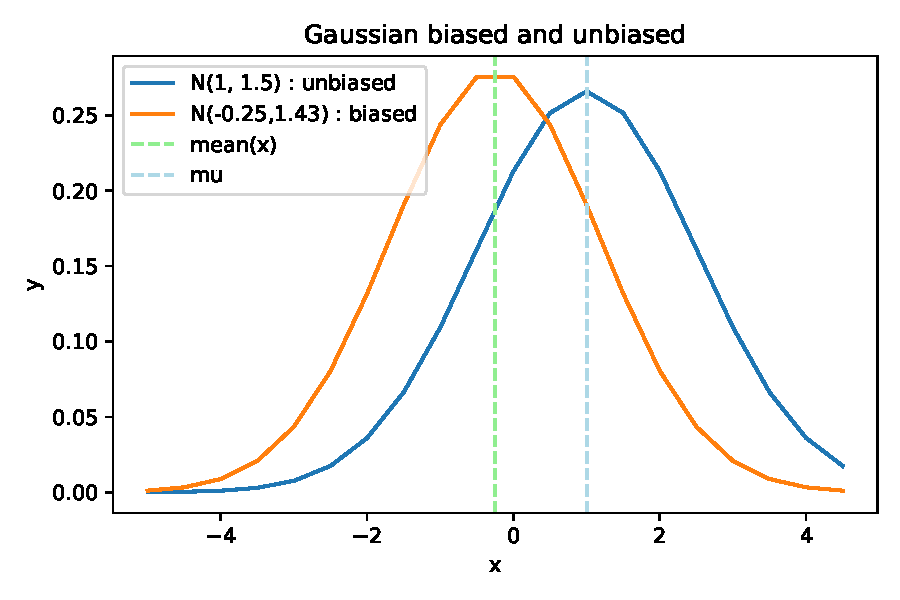
\includegraphics[scale=0.5]{images/Biased_normal_distri.pdf}
    \caption{Difference between a Biased Normal distribution and an unbiased Normal distribution}
    \label{Figure 1}
\end{figure}



\end{frame}
%%%%%%%%%%%%%%%%%%%%%%%%%%%%%%%%%%%%%%%%%%%%%%%%%%%%%%%%%%%%%%%%%%%%%%%%%%%%%%%



%%%%%%%%%%%%%%%%%%%%%%%%%%%%%%%%%%%%%%%%%%%%%%%%%%%%%%%%%%%%%%%%%%%%%%%%%%%%%%%
\begin{frame}{Characterization of the biased variance}
\vspace{0.5cm}
The expected value of the variance's biased estimator is not the variance estimator. That means :
\vspace{0.5cm}
\begin{columns}
\begin{column}[T]{.48\textwidth}
    \visible<1->{\mybold{Dimension : 1} the model writes out : \[ y = X\beta + \varepsilon\]
	where y $\sim \mathcal{N}(\mu, \sigma^2)$ and $\varepsilon \sim \mathcal{N}(0, 1)$\\
	\begin{equation*}
	  \mathbb{E}[\sigma^2]=\frac{N-1}{N}\sigma^2 \ne \sigma^2
	\end{equation*}}
	\vspace{1cm}
\end{column}
    
\begin{column}[T]{.48\textwidth}
	\visible<2->{\mybold{Dimension : k} the model writes out : \[ y = X\beta + \varepsilon\]
	where y $\sim \mathcal{N}(X\beta, \sigma^2I_k)$ and $\varepsilon \sim \mathcal{N}(0, \sigma^2I_k)$\\
	\begin{equation*}
	  \mathbb{E}[\sigma^2]=\frac{N-k}{N}\sigma^2 \ne \sigma^2
	\end{equation*}}
\end{column}
\end{columns}
\vspace{-1cm}
\visible<3->{It is an underestimation of the true variance.
We need to choose $\widehat{\sigma^2} = \frac{1}{N-k}(y-X\hat{\beta})^T(y-X\hat{\beta})$ to find an unbiased variance.}
\end{frame}
%%%%%%%%%%%%%%%%%%%%%%%%%%%%%%%%%%%%%%%%%%%%%%%%%%%%%%%%%%%%%%%%%%%%%%%%%%%%%%%



%%%%%%%%%%%%%%%%%%%%%%%%%%%%%%%%%%%%%%%%%%%%%%%%%%%%%%%%%%%%%%%%%%%%%%%%%%%%%%%
\subsection{The solution : REML}
\label{sub:The solution : REML}
%%%%%%%%%%%%%%%%%%%%%%%%%%%%%%%%%%%%%%%%%%%%%%%%%%%%%%%%%%%%%%%%%%%%%%%%%%%%%%%



%%%%%%%%%%%%%%%%%%%%%%%%%%%%%%%%%%%%%%%%%%%%%%%%%%%%%%%%%%%%%%%%%%%%%%%%%%%%%%%
\begin{frame}{The REML solution}
\vspace{1cm}
    The idea of the REML method is : \newline
    \newline
	\only<2->{1) Integrate the likelihood in relation to $\mu$} \newline
	\visible<3->{2) Calculate the log of the previous result} \newline
	\only<4->{3) Recognize the Maximum likelihood solution and the REML approach (the bias, the fee)} \newline
	\visible<5->{4) Determine the variance estimator} \newline
\end{frame}

%%%%%%%%%%%%%%%%%%%%%%%%%%%%%%%%%%%%%%%%%%%%%%%%%%%%%%%%%%%%%%%%%%%%%%%%%%%%%%%
%%%%%%%%%%%%%%%%%%%%%%%%%%%%%%%%%%%%%%%%%%%%%%%%%%%%%%%%%%%%%%%%%%%%%%%%%%%%%%%
\section{An example}
\label{sec:example}
%%%%%%%%%%%%%%%%%%%%%%%%%%%%%%%%%%%%%%%%%%%%%%%%%%%%%%%%%%%%%%%%%%%%%%%%%%%%%%%
%%%%%%%%%%%%%%%%%%%%%%%%%%%%%%%%%%%%%%%%%%%%%%%%%%%%%%%%%%%%%%%%%%%%%%%%%%%%%%%

%%%%%%%%%%%%%%%%%%%%%%%%%%%%%%%%%%%%%%%%%%%%%%%%%%%%%%%%%%%%%%%%%%%%%%%%%%%%%%%
\subsection{Data}
\label{sub:Data}
%%%%%%%%%%%%%%%%%%%%%%%%%%%%%%%%%%%%%%%%%%%%%%%%%%%%%%%%%%%%%%%%%%%%%%%%%%%%%%%

%%%%%%%%%%%%%%%%%%%%%%%%%%%%%%%%%%%%%%%%%%%%%%%%%%%%%%%%%%%%%%%%%%%%%%%%%%%%%%%
\begin{frame}{An example : Data}
    \begin{table}
        \centering
        \begin{tabular}{| c | c | c|}
        \hline
        \begin{bf} Ind \end{bf} &
        \begin{bf} Resp \end{bf} &
        \begin{bf} Treat \end{bf} \\
        \hline
        1 &  10 & 0\\
        1 & 25 & 1 \\
        2 & 3 & 0 \\
        2 &  6 & 1\\
        \hline
        \end{tabular}
    \end{table}
\vspace{1cm}
In \textit{Treat} column : $0$ means that the individual gets the treatment and $1$ means that it doesn't get the treatment.
\end{frame}
%%%%%%%%%%%%%%%%%%%%%%%%%%%%%%%%%%%%%%%%%%%%%%%%%%%%%%%%%%%%%%%%%%%%%%%%%%%%%%%

%%%%%%%%%%%%%%%%%%%%%%%%%%%%%%%%%%%%%%%%%%%%%%%%%%%%%%%%%%%%%%%%%%%%%%%%%%%%%%%
%%%%%%%%%%%%%%%%%%%%%%%%%%%%%%%%%%%%%%%%%%%%%%%%%%%%%%%%%%%%%%%%%%%%%%%%%%%%%%%
\subsection{Codes and Results}
\label{sub:Codes and Results}
%%%%%%%%%%%%%%%%%%%%%%%%%%%%%%%%%%%%%%%%%%%%%%%%%%%%%%%%%%%%%%%%%%%%%%%%%%%%%%%
%%%%%%%%%%%%%%%%%%%%%%%%%%%%%%%%%%%%%%%%%%%%%%%%%%%%%%%%%%%%%%%%%%%%%%%%%%%%%%%


%%%%%%%%%%%%%%%%%%%%%%%%%%%%%%%%%%%%%%%%%%%%%%%%%%%%%%%%%%%%%%%%%%%%%%%%%%%%%%%
\begin{frame}[fragile]{An example : Codes}

First, we use linear regression with Least Squared method (OLS)
\begin{lstlisting}
linear_reg = sm.OLS(df.Resp,df.Treat)
linear_reg_fit = linear_reg.fit()
print(linear_reg_fit.summary())
\end{lstlisting}
\vspace{0.5cm}
Then, we use mixed effects model with REML
\begin{lstlisting}
mixed_random = smf.mixedlm("Resp~Treat",df,
    groups=df['Ind'])
mixed_fit = mixed_random.fit()
print(mixed_fit.summary())
\end{lstlisting}
\end{frame}
%%%%%%%%%%%%%%%%%%%%%%%%%%%%%%%%%%%%%%%%%%%%%%%%%%%%%%%%%%%%%%%%%%%%%%%%%%%%%%%%



%%%%%%%%%%%%%%%%%%%%%%%%%%%%%%%%%%%%%%%%%%%%%%%%%%%%%%%%%%%%%%%%%%%%%%%%%%%%%%%%
\begin{frame}{An example : Results}

\begin{table}[h!]
    \centering
    \begin{tabular}{| c | c | c|c|}
        \hline
        \begin{bf} Method \end{bf} &
        \begin{bf} Log-likelihood \end{bf} &
        \begin{bf} $\sigma^2$ \end{bf} &
        \begin{bf} $\sigma_s^2$ \end{bf} \\
        \hline
        OLS linear regression &  -14.23 & 6.95 & -\\
        REML mixed effects model  & -7.89 & 6.00 & 8.15 \\
        \hline
    \end{tabular}
\end{table}
\vspace{1cm}
Both methods have the same value for the coefficients : $\beta_1=6.0$ and $\beta_2=15.5$
\end{frame}
%%%%%%%%%%%%%%%%%%%%%%%%%%%%%%%%%%%%%%%%%%%%%%%%%%%%%%%%%%%%%%%%%%%%%%%%%%%%%%%


%%%%%%%%%%%%%%%%%%%%%%%%%%%%%%%%%%%%%%%%%%%%%%%%%%%%%%%%%%%%%%%%%%%%%%%%%%%%%%%
%%%%%%%%%%%%%%%%%%%%%%%%%%%%%%%%%%%%%%%%%%%%%%%%%%%%%%%%%%%%%%%%%%%%%%%%%%%%%%%
\section{Conclusion}
\label{sec:conclusion}
%%%%%%%%%%%%%%%%%%%%%%%%%%%%%%%%%%%%%%%%%%%%%%%%%%%%%%%%%%%%%%%%%%%%%%%%%%%%%%%
%%%%%%%%%%%%%%%%%%%%%%%%%%%%%%%%%%%%%%%%%%%%%%%%%%%%%%%%%%%%%%%%%%%%%%%%%%%%%%%


%%%%%%%%%%%%%%%%%%%%%%%%%%%%%%%%%%%%%%%%%%%%%%%%%%%%%%%%%%%%%%%%%%%%%%%%%%%%%%%%
\begin{frame}{Conclusion}

The REML method allows to estimate the variance without bias.\\
\vspace{0.5cm}
The log-likelihood is different because we have a second term with the REML method : a fee. But we have the same coefficients $\beta$.
\end{frame}

%%%%%%%%%%%%%%%%%%%%%%%%%%%%%%%%%%%%%%%%%%%%%%%%%%%%%%%%%%%%%%%%%%%%%%%%%%%%%%%
\begin{frame}{Bibliography}
\nocite{*}
\printbibliography
\end{frame}
 %%%%%%%%%%%%%%%%%%%%%%%%%%%%%%%%%%%%%%%%%%%%%%%%%%%%%%%%%%%%%%%%%%%%%%%%%%%%%%

\end{document}